\documentclass[../piano_di_progetto.tex]{subfiles}

\begin{document}


\subsection{Modello incrementale}
\label{sub:incr}

Per garantire la qualità del prodotto e uno sviluppo corretto che risulterà conforme rispetto ai requisiti richiesti sul lungo periodo, il gruppo ha scelto l’\glossario{approccio
incrementale}, ovvero l’impiego di \glossario{rilasci} che mirano ad integrare nel sistema ogni volta una nuova funzionalità. Questo sistema permette di ridurre il rischio di fallimento ad ogni iterazione, producendo un nuovo valore.

Il modello di sviluppo incrementale permette di progredire tramite cicli di incremento, 
ripetuti fino a quando il prodotto non soddisferà i requisiti richiesti dal cliente. \\
Il ciclo di incremento risulta suddiviso nei seguenti passi:
\begin{enumerate}
    \item Pianificazione;
    \item Analisi dei requisiti;
    \item Progettazione;
    \item Implementazione;
    \item Test;
    \item Valutazione.
\end{enumerate}
Ogni ciclo di incremento permette lo sviluppo di una funzionalità aggiuntiva,
preventivamente discussa con il cliente durante la fase iniziale del ciclo stesso.
la ciclicità prevista dal modello incrementale facilita anche il versionamento del sistema,
tracciando modifiche nette al software.

\begin{figure}[H]
    \centering
    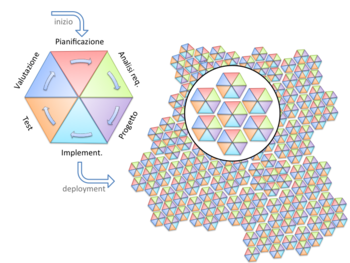
\includegraphics[scale = 0.6]{src/img/modello_incrementale.png}
    \caption{Rappresentazione del modello incrementale}
    \label{fig:logo}
\end{figure}

L'utilizzo di questo modello permette di ottenere importanti vantaggi, quali:
\begin{itemize}
    \item Maggior priorità alle funzionalità primarie, in questo modo possono essere sottoposte al cliente nel minor tempo possibile;
    \item Utilizzo dello sviluppo per incrementi successivi limita la modifica e le correzioni degli errori al singolo incremento, risultano meno onerose in termini di tempo e, di conseguenza, di costi;
    \item Le verifiche e i test sono circoscritti al singolo incremento, cioè alle nuove funzionalità;
    \item Possibilità di un maggior numero di feedback da parte del cliente, aumentando l'efficienza.
\end{itemize}

%TODO Allinenare incrementi in capitolo 3 - 4 - 5
\subsubsection{Incrementi individuati}
\label{ssub:incr_ind}

%Nei periodi di \emph{Progettezione architetturale} e \emph{Progettazione di dettaglio e codifica} sono stati individuati degli incrementi.
Di seguito viene riportato un tracciato incremento | Use case/requisito, in modo tale da comprendere più chiaramente gli UC o requisiti che verranno soddisfatti in ciascun incremento. 
%I requisiti riportati nella tabella includono tutti i requisiti figli. Tutti i requisiti non riporta-ti nella tabella sono da intendersi soddisfatti, in parte, da ogni incremento. Tali requisiti sonoreperibili all’interno del documentoAnalisi dei Requisiti.

Gli UC o i requisiti verranno sviluppati all'interno dell'incremento associato ad essi e verranno considerati soddisfatti in tutti gli incrementi sucessivi a quello di sviluppo. Gli UC e i requisiti qui riportati sono reperibili all'interno del documento \textsc{Analisi dei Requisiti v1.0.0}.
\begin{table}[!ht]
	\centering
	\begin{tabular}{|p{3cm}|p{3cm}|}
	\hline
	\rowcolor{lightgray}
	\textbf{Incremento} & \textbf{UC/Requisiti}\\
	\hline
        Incremento 1 & RVO3\\
        Incremento 2 & RVO1\\
        Incremento 3 & UC1.2  UC3 \\
        Incremento 4 & UC2.2 UC4.2.1 UC4.2.2 UC4.2.4 UC4.2.5\\
        Incremento 5 & UC1.3\\
        Incremento 6 & RxFx\\
	\hline	
	\end{tabular}
	\caption{Tabella tracciamento incremento-uc/requisiti}
\end{table}

\end{document}